\subsection{Tipo de entidad Asesor}

   \begin{description}

   \item[Definición] Se refiere al objeto del mundo real: \emph{``Tutor que
        realiza un seguimiento permanente y orientado a la optimización del
        esfuerzo de estudio de un alumno en un curso académico.''}.

   \item[Características] La entidad presenta las siguientes características:
      \begin{itemize}
         \item \textbf{Nombre:} Asesor.
         \item \textbf{Tipo:} Fuerte.
         \item \textbf{Número de atributos:} 4.
         \item \textbf{Atributo/s identificador/es principal/es:} dni\_pasaporte.
         \item \textbf{Atributo/s identificador/es alternativo/s:} correo\_electronico.
         \item \textbf{Atributo/s heredado/s:} -
      \end{itemize}

   \item[Diagrama] La figura \ref{diagramaAsesor} muestra el diagrama de la entidad.
   \item \begin{figure}[!ht]
            \begin{center}
            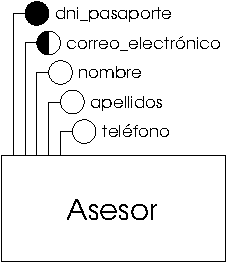
\includegraphics[]{07.Modelo_Entidad-Interrelacion/7.2.Analisis_Entidades/diagramas/asesor.pdf}
            \caption{Diagrama de la entidad Asesor.}
            \label{diagramaAsesor}
            \end{center}
         \end{figure}

   \item[Descripción de los atributos] La entidad presenta los siguientes
   atributos:

   \begin{itemize}
   \item \textbf{dni\_pasaporte}
      \begin{itemize}
         \item \textbf{Definición:} Coincide con el documento nacional de identidad o pasaporte de la persona.
         \item \textbf{Dominio:} Conjunto de caracteres alfanuméricos.
         \item \textbf{Carácter:} Obligatorio.
         \item \textbf{Ejemplo práctico:} 98765432Z.
         \item \textbf{Información adicional:} El dato lo proporciona el administrador, principal o de centro, cuando introduce al usuario asesor en el sistema. Es la clave primaria.
      \end{itemize}
   \item \textbf{correo\_electrónico}
      \begin{itemize}
         \item \textbf{Definición:} Contiene la dirección de correo electrónico de la persona.
         \item \textbf{Dominio:} Conjunto de caracteres alfanuméricos permitidos en una dirección de correo electrónico.
         \item \textbf{Carácter:} Opcional.
         \item \textbf{Ejemplo práctico:} ma1fegan@uco.es
         \item \textbf{Información adicional:} El dato lo proporciona o bien el usuario administrador, principal o de centro, cuando registra al asesor en el sistema, o bien el propio usuario asesor cuando modifica su información personal. Es la clave alterna.
      \end{itemize}
   \item \textbf{nombre}
      \begin{itemize}
         \item \textbf{Definición:} Designa el nombre de pila del usuario asesor que interviene en el sistema.
         \item \textbf{Dominio:} Conjunto de caracteres alfanuméricos.
         \item \textbf{Carácter:} Obligatorio.
         \item \textbf{Ejemplo práctico:} Nicolás Luis.
         \item \textbf{Información adicional:} El dato lo proporciona o bien el usuario administrador, principal o de centro, cuando registra al asesor en el sistema, o bien el propio usuario asesor cuando modifica su información personal.
      \end{itemize}
   \item \textbf{apellidos}
      \begin{itemize}
         \item \textbf{Definición:} Hace referencia a los apellidos del usuario asesor que interviene en el sistema.
         \item \textbf{Dominio:} Conjunto de caracteres alfanuméricos.
         \item \textbf{Carácter:}  Opcional.
         \item \textbf{Ejemplo práctico:} Fernández García.
         \item \textbf{Información adicional:} El dato lo proporciona o bien el usuario administrador, principal o de centro, cuando registra al asesor en el sistema, o bien el propio usuario asesor cuando modifica su información personal.
      \end{itemize}
   \end{itemize}

   \item[Ejemplo práctico]

   \item \begin{center}
            \begin{tabular}{ | l | l | }
            \hline
            \multicolumn{2}{ | c | }{\textbf{Tipo de entidad Asesor}} \\
            \hline
            dni\_pasaporte & 98765432Z \\
            \hline
            correo\_electrónico & ma1fegan@uco.es\\
            \hline
            nombre & Nicolás Luis\\
            \hline
            apellidos & Fernández García\\
            \hline
            \end{tabular}
         \end{center}
   \end{description}
